%%%%%%%%%%%%%%%%%%%%%%%%%%%%%%%%%%%%%%%%%%%%%%%%%%%
%
%  New template code for TAMU Theses and Dissertations starting Fall 2012.  
%  For more info about this template or the 
%  TAMU LaTeX User's Group, see http://www.howdy.me/.
%
%  Author: Wendy Lynn Turner 
%	 Version 1.0 
%  Last updated 8/5/2012
%
%%%%%%%%%%%%%%%%%%%%%%%%%%%%%%%%%%%%%%%%%%%%%%%%%%%
%%%%%%%%%%%%%%%%%%%%%%%%%%%%%%%%%%%%%%%%%%%%%%%%%%%%%%%%%%%%%%%%%%%%%%
%%                           SECTION V
%%%%%%%%%%%%%%%%%%%%%%%%%%%%%%%%%%%%%%%%%%%%%%%%%%%%%%%%%%%%%%%%%%%%%


\chapter{\uppercase{Experiments, Results and Analysis}}

To verify and demonstrate the scalability that the user application could achieve through utilizing DMAT, we conducted a series of experiments, including data transposing and 3D stencil calculation, an overlapping-calculation application. 

\section{3D Volume Transposing}

\subsection{Use Case}

This section presents the experiments of the 3D transposing problem mentioned in previous chapter. The dataset we used for transposing (from I  to J direction) experiment is a 300GB seismic 3D volumetric data, which is 31017 x 97223 x 31 in I x J x K direction with float data type. 
We design the experiment to verify the performance of transposing is scalable and is mainly affected by the data distribution configuration and the amount of available hardware resource(the total count of cores).

\subsection{Statistics and Analysis}

\paragraph{Scalability to the Number of CPU Cores}

We conducted the transposing experiment on a cluster with 24 nodes, each node has 12 cores(24 cores in Hyper-threading) and 48GB available DRAM. The total CPU cores is 288(576 in Hyper-threading). Figure \ref{TestStat} shows the performance metrics of this experiment. The \emph{x} in \emph{Transpose[x]} stands for the aggregation parameter we applied on the dataset. As mentioned in previous chapter, the value of aggregation parameter \emph{x} determines the number of planes of each partitions thus to control the size of each data split. 

\begin{figure}[h]
\centering
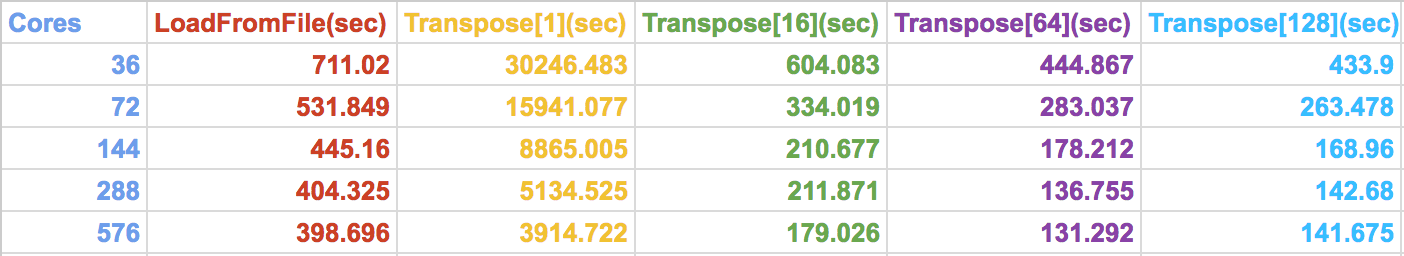
\includegraphics[scale=0.6]{figures/TestStat.png}\\
\caption{Transposing Experiment Statistics on Cluster with 288(576) cores.}\label{TestStat}
\end{figure}

From the metrics, we got two bar chart which shows the time consuming for the transposing of aggregated and non-aggregated data. It clearly demonstrates that the performance scalability on dimension of the count of CPU cores is promised, as shown in Figure \ref{PerfTestCoresNoAgg} and  Figure \ref{PerfTestCoresAgg}.  The performance difference between the transposing on aggregated and non-aggregated seismic volume data will be addressed in the following paragraph.

\begin{figure}[ht]
\centering
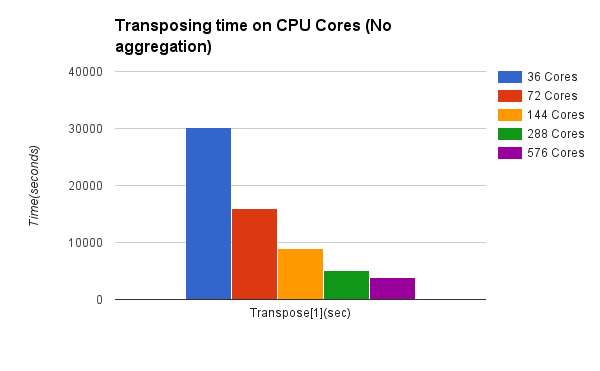
\includegraphics[scale=0.7]{figures/PerfTestCoresNoAgg.png}\\
\caption{Transposing Time on CPU Cores without Aggregation}\label{PerfTestCoresNoAgg}
\end{figure}

\begin{figure}[h]
\centering
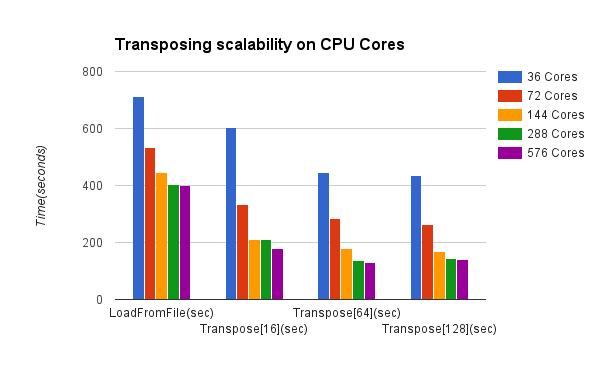
\includegraphics[scale=0.7]{figures/PerfTestCoresAgg.png}\\
\caption{Transposing Time on CPU Cores with Aggregation.}\label{PerfTestCoresAgg}
\end{figure}


\paragraph{Scalability to the Fashion of Data Distributions}

There is another important factor, the data distribution fashion, will also affect the performance of transposing. As we mentioned in previous section, the transposing program will perform some shuffle operation on volumetric RDD. Shuffle operations \cite{SparkShuffle} is Spark's mechanism for re-distributing data so that it could change the data organization across partitions. This typically involves copying data across executors and nodes, which makes the shuffle a complex and costly operation. To reduce the shuffle costs, we could aggregate the SeismicRDD data splits to reduce the number of partitions thus to decrease the amount of data need to exchange during 3D transposing on each data split. Figure \ref{PerfTestAgg} shows the performance improvement when we increasing the aggregated planes number (\emph{x} in \emph{Transpose[x]}) of each data distribution. 

\begin{figure}[h]
\centering
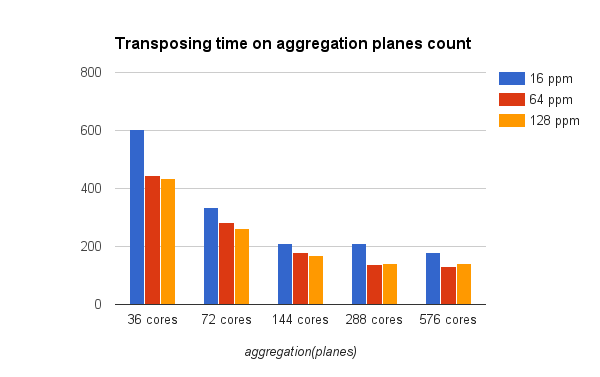
\includegraphics[scale=0.7]{figures/PerfTestAgg.png}\\
\caption{Transposing Time on Aggregated Planes(ppm: planesPerMap).}\label{PerfTestAgg}
\end{figure}

However, the curve of performance trends to flat when the aggregation increases to a higher level. That is caused by the performance trade-off when reducing the distribution partitions, which will lead to a lower cluster CPU cores utilizing rate. Therefore, to achieve a reasonable performance for transposing operation, developer needs to considerate the trade-off between distribution configurations and data shuffling. 

Figure \ref{NMONCPU} and Figure \ref{NMONMEM} show the CPU utilization and memory usage of each node when the transposing experiment was running on the cluster. These system statistic visualization views were generated by a free software NMONVisualizer \cite{NMONVisualizer}, which is a Java GUI tool for analyzing Nmon performance files.
% from both AIX and Linux. 
%It also parses IOStat files, IBM verbose GC logs, Windows Perfmon and ESXTop CSV data and JSON data.

\begin{figure}[h]
\centering
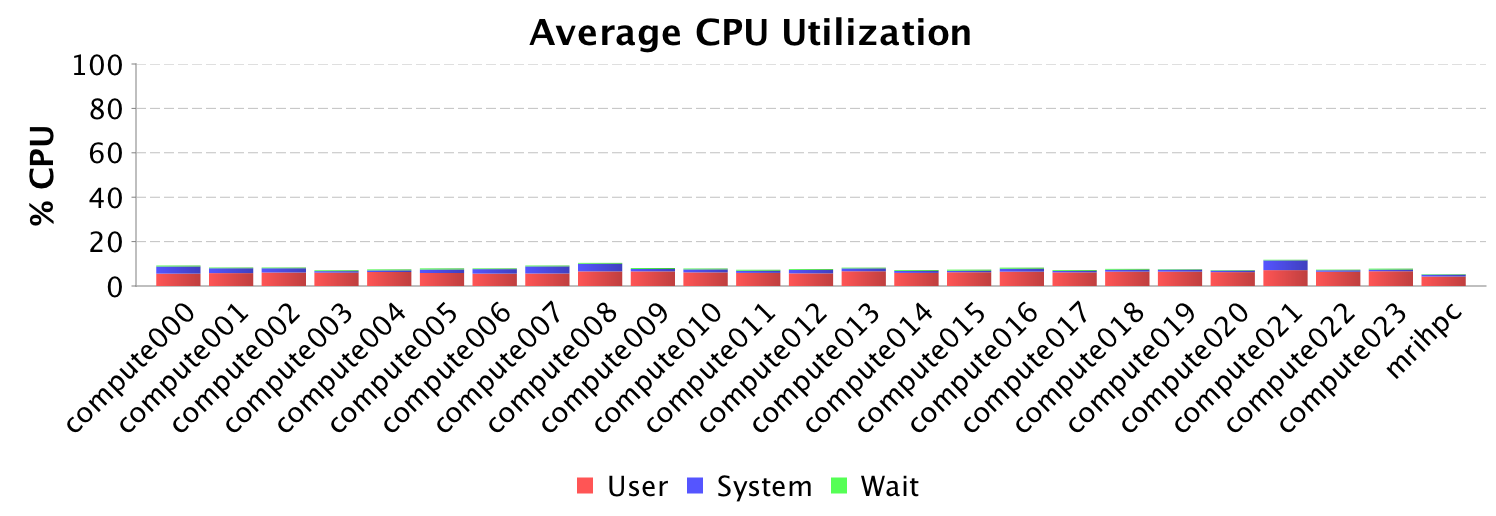
\includegraphics[scale=0.6]{figures/NMONCpu.png}\\
\caption{CPU utilization statistics from NMONVisualier.}\label{NMONCPU}
\end{figure}

\begin{figure}[h]
\centering
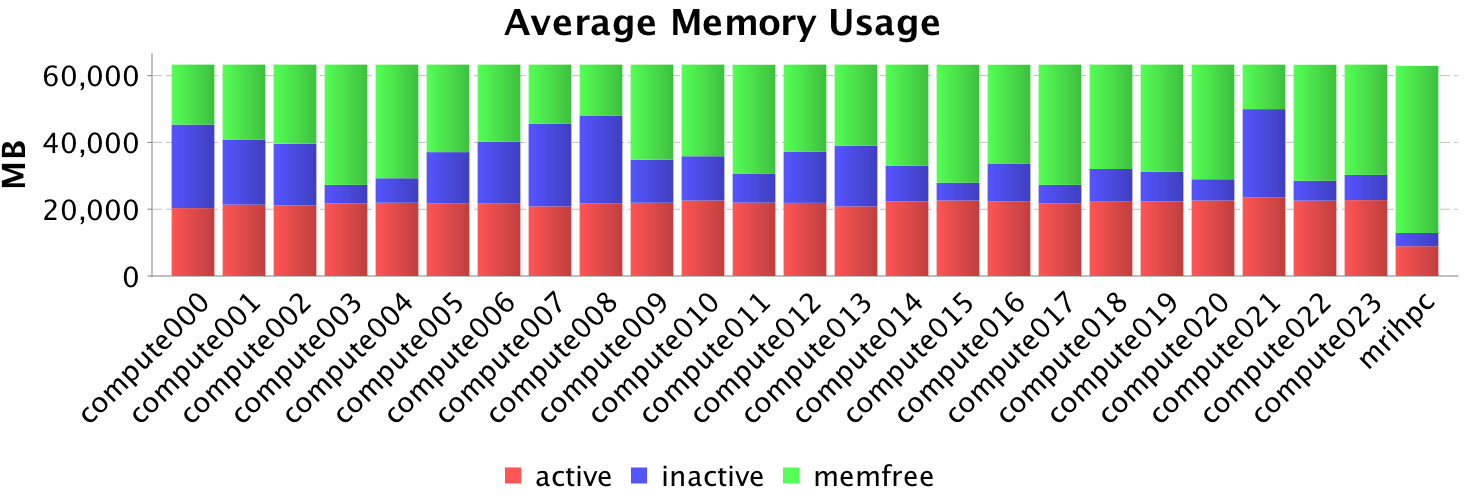
\includegraphics[scale=0.6]{figures/NMONMemory.png}\\
\caption{DRAM utilization statistics from NMONVisualier.}\label{NMONMEM}
\end{figure}

\paragraph{Cross-Verification on the Third-party Cloud Platform: XSEDE Cluster}

To further verify the scalability, we also setup the same experiment on the XSEDE supercomputing cluster \cite{XSEDE}. We request 44 nodes from XSEDE cluster, which has 12 cores in each node. Figure \ref{XSEDETestStat} shows the result statistics of this experiment. As shown in Figure \ref{XSEDETest}, we conduct the experiment to test the scalability of case transposing the same volumetric data from I to J direction, aggregation is 16 planes, and the result also verified the scalability of this distributed application.

\begin{figure}[h]
\centering
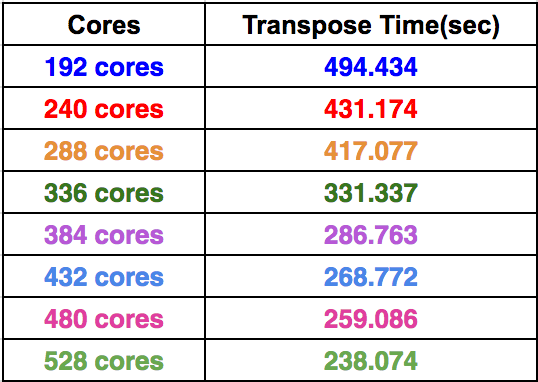
\includegraphics[scale=0.6]{figures/XSEDETestStat.png}\\
\caption{The Transposing Performance Statistics on XSEDE Cluster}\label{XSEDETestStat}
\end{figure}

\begin{figure}[h]
\centering
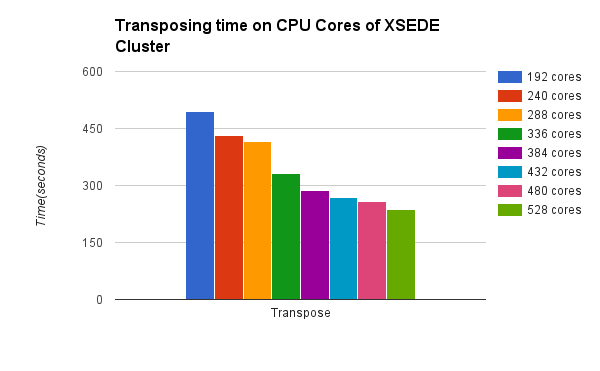
\includegraphics[width=0.8\textwidth]{figures/XSEDETest.png}\\
\caption{The Performance Scalability of Transposing on XSEDE Cluster }\label{XSEDETest}
\end{figure}


\section{3D Stencil Application}

\subsection{Use Case}

Stencil computations are most commonly used in context of scientific and engineering applications such as signal and image processing, computer simulations etc.
Stencil itself represents an iterative kernel that updates array elements according to fixed pattens \cite{StencilWiki}. The optimization on stencil computation has been well studied in \cite{Han2011PADS},\cite{Nguyen2010Blocking} and \cite{Datta2008Stencil}. 
However, most of these optimizations focus on single node implementation with GPU or multi-core CPUs. In \cite{YanMasterThesis}, \cite{7363985} and \cite{7396203}, the authors provide a parallel implementation with Spark RDD, which gives a scalable solution for big data that can not host on a single node. 
%The approach simplifies the development efforts by underline complicate data distribution problem. 
In this experiment, we use the defined parallel templates in DMAT to implement stencil computations, and test their performance as well as scalability.

\subsection{Statistics and Analysis}

The dataset we choose to conduct our experiment is called Penobscot dataset, which is actual seismic image data with 3D dimension size 600x481x1501. 
The cluster consists of 8 nodes, in which one is management node and other 7 nodes are computation nodes. Each node was equipped with Intel Xeon E5-2690 Sandy Bridge CPU (2.9 GHz, 16 Cores or 32 Cores with Hyper-threading support), 128GB DDR3 memory and are inter-connected with 1GB ethernet. 
JDK 1.8.0\_40, Hadoop 2.5.1 and Spark 1.6.1 are used for compiling and running applications. Wall clock is used to get the running time, and Nmon/Spark Web UI are used for performance analysis.

For the algorithm, we use a variant of Jacobi iteration, which uses a 3D subvolume with dimension size of 3x3x3 as input, and in the computation, each new output value at (i, j, k) is the average value of 26 surrounding samples plus itself. In the case of 3x3x3 subvolume, the overlap area is 1. 
For the sequential codes, we just split the big 3D data file into small partition and each partition includes several 2D planes (the overlap between partition is one 2D plane), and then use 3 nested loops to compute the average value. 
For the parallel codes using DMAT, we use the overlapped template, which specify parameters both in I and J directions. 
Different configurations of cores and numbers of planes in each partition are set to check performance and scalability. 
The numbers of cores (28, 56, 112, 224) are used for each test case respectively to verify the scalability of parallel codes. 
Within each configuration of cores, we use different combinations of dimension size (1, 2, 4, 8) in I and J directions. For instance, I(4) and J(2) mean that the dimension size of input subvolume 6x4, which comes from (4+2*1)x(2+2*1) in the case of overlap is 1, which is shown in Figure \ref{StencilData}

\begin{figure}[h]
\centering
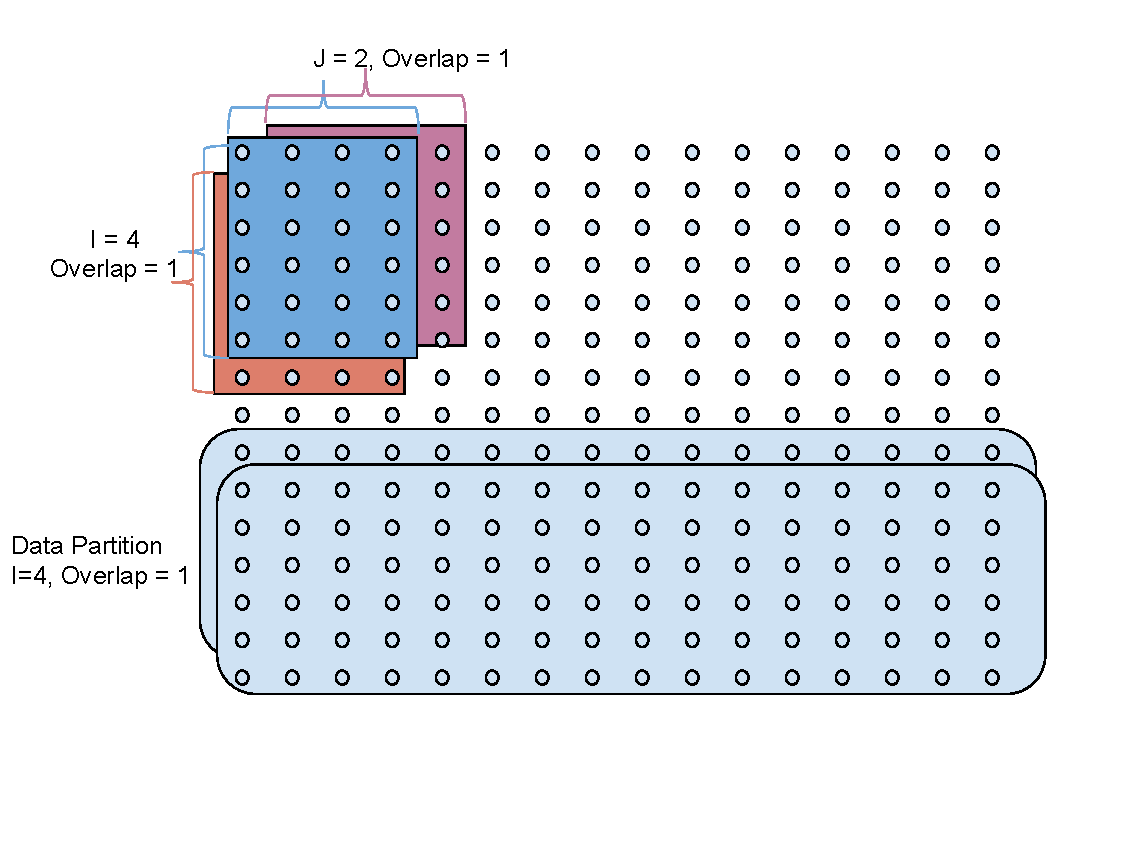
\includegraphics[scale=0.7]{figures/StencilData.pdf}\\
\caption{The Data Distributation and Input of Overlaop Template}
\label{StencilData}
\end{figure}

Figure \ref{Stencil28} and Figure \ref{Stencil224} show the speed up of parallel codes on Spark with 28 cores and 224 cores to the sequential codes respectively. 
From these two figures, the changes on number of \emph{J} have little impact on the performance, because it does not change the number of planes in each partition and the number of partitions. In the template implementation, two nested loops are used for feeding the input of each stencil kernel. However, the change on number of \emph{I} tells how the SDK distributes the data and the number of partitions, thus will determine how many tasks are need to finish that stage of in the job, and each task need to be assinged one thread or one core to undertake the computation.
In the case that size of \emph{I} is 1, it gets the best speed up in all test cases. It seems to be abnormal that the performance decreases from 1 plane of I to 2 planes of I. Increasing I will enlarge the size of each partition as shown in Figure \ref{StencilData}, however, the amount of computations keeps constant. In this stencil computation, we iterate several times to reach the balance. 
At the beginning of each loop, the data need to be repartitioned based on the overlap parameter, since the latest edge data need to be updated to each partition for next iteration. In the process of repartition, it needs to get planes at the left and right edge, sort them by key and zip with original latest results, which trigger data shuffle in Spark. The bigger the size of partitions is, the more time it takes to shuffle them. The 'Shuffle Read Blocked Time' increases drastically from 1 plane of I to 2 planes of I, which accounts for the performance decreasing. 
Figure \ref{StencilBest} shows the best speedup with different configurations of cores, in which the scalability is obvious while increasing the number of cores.

\begin{figure}[h]
\centering
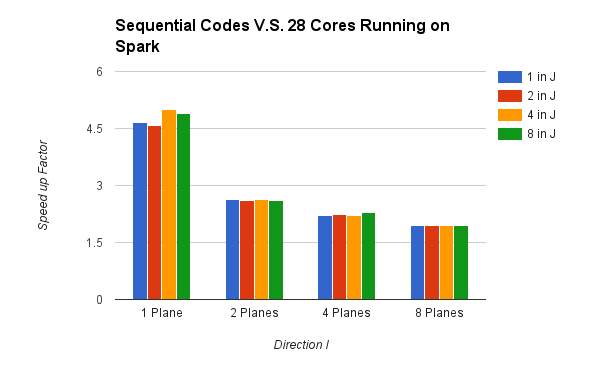
\includegraphics[scale=0.7]{figures/Stencil28.png}\\
\caption{The Speedup of Parallel Template Codes with 28 Cores to Sequential Codes}
\label{Stencil28}
\end{figure}

\begin{figure}[h]
\centering
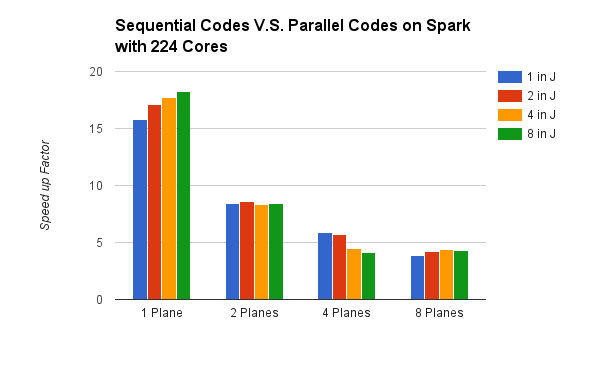
\includegraphics[scale=0.7]{figures/Stencil224.png}\\
\caption{The Speedup of Parallel Template Codes with 224 Cores to Sequential Codes}
\label{Stencil224}
\end{figure}

\begin{figure}[h]
\centering
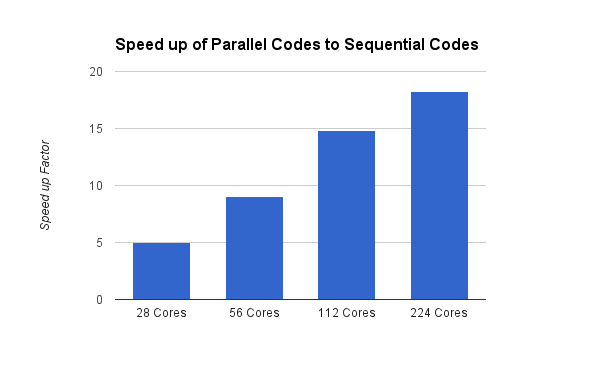
\includegraphics[scale=0.7]{figures/StencilBest.png}\\
\caption{The Best Speedup of Parallel Templates for Stencil Computation}
\label{StencilBest}
\end{figure}


